\subsection{First Order Systems of Differential Equations}
\subsubsection{Converting to First Order}
A system of differential equations is where we are dealing with multiple dependent variables, $x_1(t), x_2(t), \ldots, x_n(t)$.\\
In some cases, each system can be solved independently, making them easy to solve.\\
Ex: solve $\displaystyle{\eqnsystem{x_1'=x_2-x_1+t\\x_2'=x_2}}$
\begin{align*}
    &x_2=C_2e^{t}\\
    &x_1'=C_2e^t-x_1+t\\
    &x_1'+x_1=C_2e^t+t\\
    &r=e^t\\
    &x_1=r^{-1}\int rgdt\\
    &x_1=e^{-t}\int e^t(C_2e^t+t)dt\\
    &\int te^tdt\\
    &u=t\Ra du=dt\\
    &dv=e^tdt\Ra v=e^t\\
    &\int te^tdt=te^t-\int e^tdt=te^t-e^t+C\\
    &x_1=e^{-t}\brround{\frac{C_2}{2}e^{2t}+te^t-e^t+C}\\
    &x_1=\frac{C_2}{2}e^t+t-1+C_1e^{-t}\\
    &\vec{x}=\matrixx{\frac{C_2}{2}e^t+t-1+C_1e^{-t}\\C_2e^t}
\end{align*}
This is quite uncommon though. In most cases we will be required to express the system as a matrix and solve using linear algebra methods.\\
A general first order system of differential equations is given by
$$\frac{d\vec{x}}{dt}=A\vec{x}+\vec{f}(t)$$
Many systems of equations can be represented as first order systems.\\
Ex: express $y''-4y'+3y=0$ as a first order system.
\begin{align*}
    &x_1=y,\ x_2=y'\\
    &x_1'=x_2\\
    &x_2'-4x_2+3x_1=0\Ra x_2'=4x_2-3x_1\\
    &\matrixx{x_1'\\x_2'}=\matrixx{0&1\\-3&4}\matrixx{x_1\\x_2}\\
    &\vec{x}'=\matrixx{0&1\\-3&4}\vec{x}
\end{align*}
Ex2: express the system $\displaystyle{\eqnsystem{m_1x_1''+cx_1'=-k_1x_1+k_2(x_2-x_1)\\m_2x_2''+cx_2'=-k_2(x_2-x_1)-k_3x_2}}$ as a first order system.
\begin{align*}
    &\text{let }u_1=x_1,\ u_2=x_1',\  u_3=x_2,\ u_4=x_2'\\
    &\eqnsystem{m_1u_2'+cu_2=-ku_1+k_2u_3-k_2u_1\\m_2u_4'+cu_4=-k_2u_3+k_2u_1-k_3u_3\\u_1'=u_2\\u_3'=u_4}\Ra \eqnsystem{u_2'=\frac{1}{m_1}\brround{k_2u_3-(k_1+k_2)u_1-cu_2}\\u_4'=\frac{1}{m_2}\brround{k_2u_1-(k_2+k_3)u_3-cu_4}\\u_1'=u_2\\u_3'=u_4}\\
    &\frac{d\vec{u}}{dt}=\matrixx{0&1&0&0\\-\frac{k_1+k_2}{m_1}&-\frac{c}{m_1}&\frac{k_2}{m_1}&0\\0&0&0&1\\\frac{k_2}{m_2}&0&-\frac{k_2+k_3}{m_2}&-\frac{c}{m_2}}\vec{u}
\end{align*}
\subsubsection{Linear Systems of Differential Equations}
These are differential equations in the form of $\frac{d\vec{x}}{dt}=A\vec{x}$ and can be solved with the following method:
\begin{enumerate}
    \item Set $\frac{d\vec{x}}{dt}=A\vec{x}$ and find the matrix $A$
    \item Find eigenvalues and eigenvectors of $A$
    \item Write the general solution
    \item Express the general solution as $\vec{x}(t)=c_1e^{\lambda_1t}\vec{v}_1+c_2e^{\lambda_2t}\vec{v}_2+\cdots$
    \item If imaginary, express conjugate pairs as $c_1\vec{P}(t)+c_2\vec{Q}(t)$ where $\vec{P}(t)=\Re\brround{e^{\alpha t}\vec{v}_1(\cos(\beta t)+i\sin(\beta t))}$ and $\vec{Q}(t)=\Im\brround{e^{\alpha t}\vec{v}_1(\cos(\beta t)+i\sin(\beta t))}$
    \item Use the initial conditions to solve for the coefficients, $\vec{c}$
\end{enumerate}
\textbf{Real Eigenvalues}\\
This is the most general case where the number of eigenvalues matches the size of the matrix. In this case the general solution can be expressed as
$$\vec{x}(t)=c_1e^{\lambda_1 t}\vec{v}_1+c_2e^{\lambda_2 t}\vec{v}_2+\cdots$$
\begin{align*}
    \text{Ex: }&\eqnsystem{\frac{dx_1}{dt}=x_1+x_3,\,x_1(0)=1\\\frac{dx_2}{dt}=x_2,\,x_2(0)=1\\\frac{dx_3}{dt}=x_1+x_3,\,x_3(0)=0}\\
    &\vec{x}=\matrixx{x_1(t)\\x_2(t)\\x_3(t)}\\
    &\frac{d\vec{x}}{dt}=A\vec{x}\Ra A=\matrixx{1&0&1\\0&1&0\\1&0&1},\,\vec{x}(0)=\matrixx{1\\1\\0}\\
    &\text{Eigen-analysis gives}\\
    &\eqnsystem{\lambda_1=0,\,\vec{v}_1=\matrixx{-1&0&1}^T\\\lambda_2=1,\,\vec{v}_2=\matrixx{0&1&0}^T\\\lambda_3=2,\,\vec{v}_3=\matrixx{1&0&1}^T}\\
    &\vec{x}(t)=c_1e^{0t}\matrixx{-1\\0\\1}+c_2e^t\matrixx{0\\1\\0}+c_3e^{2t}\matrixx{1\\0\\1}\\
    &c_1\matrixx{-1\\0\\1}+c_2\matrixx{0\\1\\0}+c_3\matrixx{1\\0\\1}=\matrixx{1\\1\\0}\Ra \matrixx{-1&0&1\\0&1&0\\1&0&1}\matrixx{c_1\\c_2\\c_3}\leadsto\vec{c}=\matrixx{-\frac{1}{2}\\1\\\frac{1}{2}}\\
    &\vec{x}(t)=-\frac{1}{2}\matrixx{-1\\0\\1}+e^t\matrixx{0\\1\\0}+\frac{1}{2}e^{2t}\matrixx{1\\0\\1}=\matrixx{\frac{1}{2}+\frac{1}{2}e^{2t}\\e^t\\-\frac{1}{2}+\frac{1}{2}e^{2t}}
\end{align*}

\textbf{Complex Eigenvalues}\\
This case will have the same general solution but because of the imaginary components, it can be simplified using Euler's equation. We can express any conjugate pairs as $c_1\vec{P}(t)+c_2\vec{Q}(t)$ where
$$\vec{P}(t)=\Re\brcurly{e^{\alpha t}\vec{v}_1(\cos(\beta t)+i\sin(\beta t))}\text{ and }\vec{Q}(t)=\Im\brcurly{e^{\alpha t}\vec{v}_1(\cos(\beta t)+i\sin(\beta t))}$$
\begin{align*}
    \text{Ex: }&\frac{d\vec{x}}{dt}=A\vec{x},\,A=\matrixx{0&0&3\\1&0&-1\\0&1&3}\\
    &\text{eigen-analysis gives}\\
    &\eqnsystem{\lambda_1=3,\,\vec{v}_1=\matrixx{1&0&1}^T\\\lambda_2=i,\,\vec{v}_2=\matrixx{-3i&-3+i&1}^T\\\lambda_3=-i,\,\vec{v}_3=\matrixx{3i&-3-i&1}^T}\\
    &\text{Real part: }e^{\lambda_1t}\vec{v}_1=e^{3t}\matrixx{1\\0\\1}\\
    &\text{Imaginary part: }e^{\lambda_2t}\vec{v}_2=e^{it}\matrixx{-3i\\-3+i\\1}=(\cos(t)+i\sin(t))\matrixx{-3i\\-3+i\\1}\\
    &=\matrixx{3\sin(t)-3i\cos(t)\\-3\cos(t)+i\cos(t)-3i\sin(t)-\sin(t)\\\cos(t)+i\sin(t)}\\
    &\vec{P}(t)=\Re\matrixx{3\sin(t)-3i\cos(t)\\-3\cos(t)+i\cos(t)-3i\sin(t)-\sin(t)\\\cos(t)+i\sin(t)}=\matrixx{3\sin(t)\\-3\cos(t)-\sin(t)\\\cos(t)}\\
    &\vec{Q}(t)=\Im\matrixx{3\sin(t)-3i\cos(t)\\-3\cos(t)+i\cos(t)-3i\sin(t)-\sin(t)\\\cos(t)+i\sin(t)}=\matrixx{-3\cos(t)\\\cos(t)-3\sin(t)\\\sin(t)}\\
    &\vec{x}(t)=c_1e^{3t}\matrixx{1\\0\\1}+c_2\matrixx{3\sin(t)\\-3\cos(t)-\sin(t)\\\cos(t)}+c_3\matrixx{-3\cos(t)\\\cos(t)-3\sin(t)\\\sin(t)}
\end{align*}

\textbf{Repeated Eigenvalues}\\
With repeated eigenvalues, we may not have enough eigenvectors to capture the solution space. We consider the size of the matrix to be called the \textit{algebraic multiplicity} of the system and the number of eigenvectors the \textit{geometric multiplicity} of the system.\\
In the case where the geometric multiplicity is the same as the algebraic multiplicity, the solution will follow the from the regular, non-repeated, case.
\begin{align*}
    \text{Ex: }&\vec{x}'=\matrixx{2&0\\0&2}\vec{x}\\
    &\lambda=2\\
    &A-\lambda I=\matrixx{0&0\\0&0}\to\vec{v}_1=\matrixx{1\\0},\ \vec{v}_2=\matrixx{0\\1}\\
    &\vec{x}=c_1e^{2t}\matrixx{1\\0}+c_2e^{2t}\matrixx{0\\1}\\
    &\vec{x}=e^{2t}\matrixx{c_1\\c_2}
\end{align*}
When the algebraic and geometric multiplicities are not equal, we can introduce generalized eigenvectors.\\
$\vec{v}_1$ is an eigenvector if $(A-\lambda I)\vec{v}_1=0$.\\
Similarly, $\vec{v}_2$ is a generalized eigenvector of $\vec{v}_1$ if $(A-\lambda I)\vec{v}_2=\vec{v}_1$\\
In the most general sense, we can determine if $\vec{v}$ is a generalized eigenvector if
$$(A-\lambda I)^k\vec{v}\neq\vec{0}\text{ and }(A-\lambda I)^{k+1}\vec{v}=\vec{0}$$
Note that the choice of generalized eigenvectors will always be somewhat arbitrary, as there are infinitely many choices.\\
The general solution for multiple eigenvalues will resemble the form
$$\vec{x}(t)=c_1e^{\lambda_1 t}\vec{v}_1+c_2e^{\lambda_1 t}\brround{\vec{v}_k+t\vec{v}_{k-1}+\frac{t}{2}\vec{v}_{k-2}+\cdots+\frac{t^{k-2}}{(k-2)!}\vec{v}_2+\frac{t^{k-1}}{(k-1)!}\vec{v}_1}$$
\begin{align*}
    \text{Ex: }&\vec{x}'=\matrixx{5&-3\\3&-1}\vec{x}\\
    &\det A=4,\ \trace A=4\Ra \lambda=2\\
    &\matrixx{3&-3\\3&-3}\to\vec{v}_1=\matrixx{1\\1}\\
    &\matrixx{3&-3\\3&-3}\vec{v}_2=\matrixx{1\\1}\Ra\vec{v}_2=\matrixx{\frac{1}{3}\\0}\\
    &\vec{x}=c_1e^{2t}\matrixx{1\\1}+c_2e^{2t}\brround{t\matrixx{1\\1}+\matrixx{\frac{1}{3}\\0}}
\end{align*}
\begin{align*}
    \text{Ex2: }&\vec{x}'=\matrixx{0&1&0\\0&0&1\\0&0&0}\vec{x}\\
    &\lambda=0,\ \vec{v}_1=\matrixx{1\\0\\0}\\
    &\matrixx{0&1&0\\0&0&1\\0&0&0}\vec{v}_2=\matrixx{1\\0\\0}\to \vec{v}_2=\matrixx{0\\1\\0}\\
    &\matrixx{0&1&0\\0&0&1\\0&0&0}\vec{v}_3=\matrixx{0\\1\\0}\to\vec{v}_3=\matrixx{0\\0\\1}\\
    &\vec{x}=c_1\matrixx{1\\0\\0}+c_2\brround{\frac{t^2}{2}\matrixx{1\\0\\0}+t\matrixx{0\\1\\0}+\matrixx{0\\0\\1}}
\end{align*}
\subsubsection{LCR Circuits}
Recall, $V_C=\frac{q}{C}\Ra\frac{dV_C}{dt}=\pm\frac{i}{C}$ and $\frac{dI}{dt}=\pm\frac{E}{L}$\\
where $V$ is the voltage of the capacitor, $i$ is the current through the capacitor, $E$ is the voltage of the inductor, and $I$ is the current throuh the inductor. $C$ and $L$ are the capacitance and inductance. 
\begin{enumerate}
    \item Write voltage and current equations
    \item Express $i$ and $E$ in terms of $I$ and $V$
    \item Write differential equations of form $\frac{dV}{dt}=\pm\frac{i}{C}$ and $\frac{dI}{dt}=\pm\frac{E}{L}$
    \item Express the system of differential equations in matrix form
    \item Solve differential equation for various $V(t)$ and $I(t)$
\end{enumerate}
Ex:\\
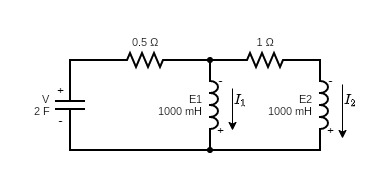
\includegraphics[scale=0.8]{Images/LinearAlgebraPictures/LCRcircuitEx.jpg}
\begin{align*}
    &\text{Voltage equations}\\
    &0.5i_1-E_1-V=0\\
    &i_2-E_2+E_1=0\\
    &\text{current equations}\\
    &I_1=i_1-i_2\\
    &I_2=i_2\\
    &\text{writing expressions in terms of }V,\,I_1,\,I_2\\
    &i_2=I_2\\
    &i_1=I_1+i_2=I_1+I_2\\
    &E_1=0.5i_1-V=0.5I_1+0.5I_2-V\\
    &E_2=i_2+E_1=0.5I_1+1.5I_2-V\\
    &\text{Differential equations for }V,\,I_1,\,I_2\\
    &\frac{dV}{dt}=-\frac{i_1}{C}=-\frac{i_1}{2}=-\frac{(I_1+I_2)}{2}\\
    &\frac{dI_1}{dt}=-\frac{E_1}{L}=-\frac{E_1}{1}=-0.5I_1+0.5I_2-V\\
    &\frac{dI_2}{dt}=-\frac{E_2}{L}=-\frac{E_2}{1}=-0.5I_1+1.5I_2-V\\
    &\frac{d}{dt}\matrixx{V\\I_1\\I_2}=\matrixx{0&-\frac{1}{2}&-\frac{1}{2}\\1&-\frac{1}{2}&-\frac{1}{2}\\1&-\frac{1}{2}&-\frac{3}{2}}\matrixx{V\\I_1\\I_2}\\
    &\text{eigenvalues and eigenvectors}\\
    &\lambda_1=\frac{-1+i}{2},\,\vec{v}_1=\matrixx{1&-i&1}^T\\
    &\lambda_2=\frac{-1-i}{2},\,\vec{v}_2=\matrixx{1&i&1}^T\\
    &\lambda_3=-1,\,\vec{v}_3=\matrixx{1&0&2}^T\\
    &\text{general solution}\\
    &\matrixx{V(t)\\I_1(t)\\I_2(t)}=c_1e^{\lambda_1t}\vec{v}_1+c_2e^{\lambda_2t}\vec{v}_2+c_3e^{\lambda_3t}\vec{v}_3\\
    &\matrixx{V(t)\\I_1(t)\\I_2(t)}=c_1e^{-t/2}\matrixx{\cos\brround{\frac{t}{2}}\\\sin\brround{\frac{t}{2}}\\\cos\brround{\frac{t}{2}}}+c_2e^{-t/2}\matrixx{\sin\brround{\frac{t}{2}}\\-\cos\brround{\frac{t}{2}}\\\sin\brround{\frac{t}{2}}}+c_3e^{-t}\matrixx{1\\0\\2}\\
    &\to\,\vec{c}\text{ can be solved from initial conditions}
\end{align*}
This particular example would show damped oscillations in the circuit.
\subsubsection{Phase Portraits}
Phase portraits are a snapshot of the vector field and phase lines formed by the solution to a system of differential equations.\\
Ex: $\vec{x}'=\matrixx{1&1\\0&2}\vec{x}$
\begin{align*}
    &\lambda=1,2,\ \vec{v}_1=\matrixx{1\\0},\ \vec{v}_2=\matrixx{1\\1}\\
    &\vec{x}=c_1e^{t}\matrixx{1\\0}+c_2e^{2t}\matrixx{1\\1}\\
    &\lim_{t\to\infty}\vec{x}=\infty\text{ parallel to }\matrixx{1\\1}\\
    &\lim_{t\to\infty}\vec{x}=0\text{ parallel to }\matrixx{1\\0}
\end{align*}
\centerline{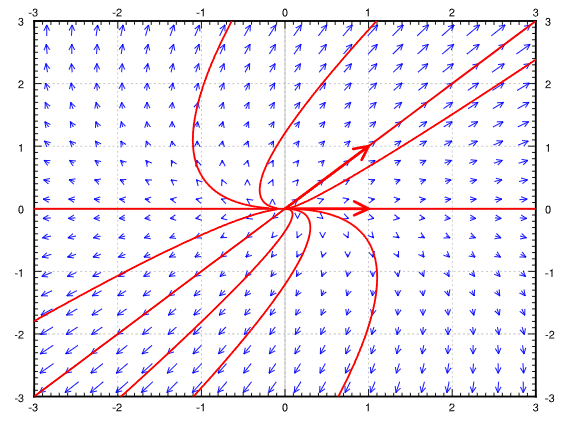
\includegraphics[scale=0.8]{Images/ODEPictures/phasePortrait1.png}}
If we take the system $\vec{x}'=\matrixx{-1&-1\\0&-2}$, we get the same eigenvectors as before but with $\lambda=-1,-2$. This gives the plot\\
\centerline{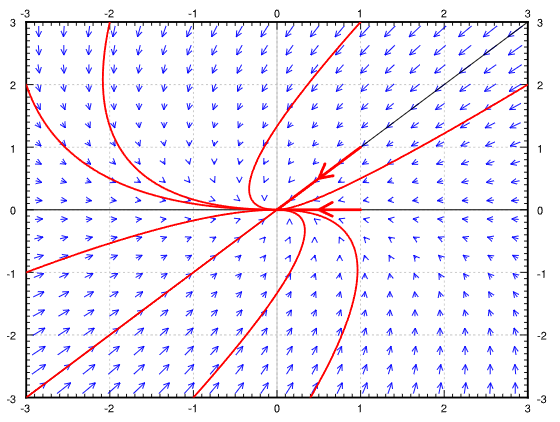
\includegraphics[scale=0.8]{Images/ODEPictures/phasePortrait2.png}}
where the system tends toward the origin.\\
We can also have cases where the eigenvalues are of opposite signs which will form a saddle\\
\centerline{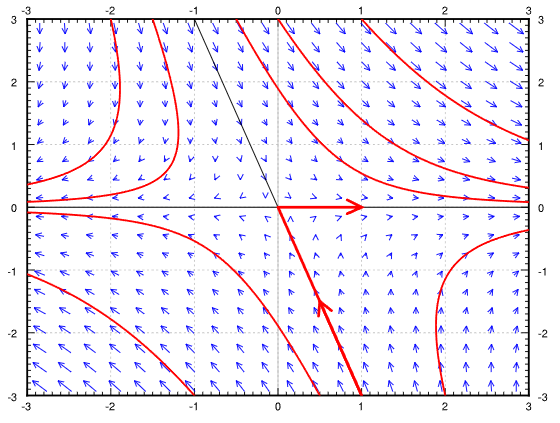
\includegraphics[scale=0.8]{Images/ODEPictures/phasePortrait3.png}}
The cases with repeated eigenvalues will react similarly to the first two examples but with the all the lines evenly diverging or converging to/from the origin.\\
In the case of complex eigenvalues, if we have no real component, the phase portrait will follow an elliptical orbit about the origin.\\
\centerline{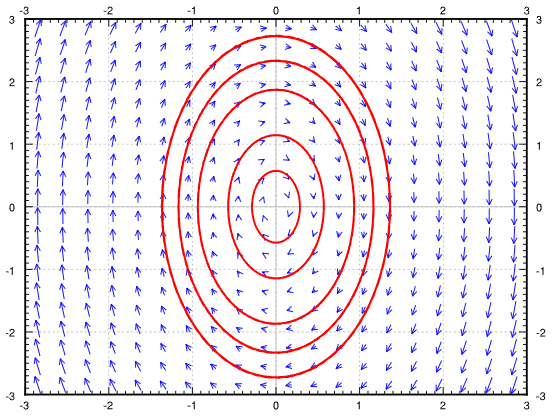
\includegraphics[scale=0.8]{Images/ODEPictures/phasePortrait4.png}}
If the eigenvalues are complex and do have a real part, they will form a spiral. For a positive real part, it will spiral out toward infinity, and a negative real part will give a spiral toward the origin.\\
\centerline{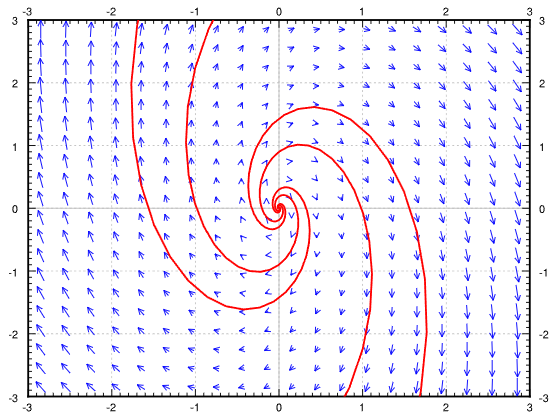
\includegraphics[scale=0.8]{Images/ODEPictures/phasePortrait5.png}}
Based on the phase portraits, we can classify the stability of different solutions\\
\begin{tabular}{l|l}
    Eigenvalues & Behavior\\
    \hline
     both real and positive & unstable source\\
    both real and negative & stable sink\\
    both real with opposite signs & unstable saddle\\
    complex with no real part & center point/ellipses\\
    complex with positive real part & spiral source\\
    complex with negative real part & spiral sink
\end{tabular}

\subsubsection{Nonhomogeneous Equations}
These are systems in the form of
$$\vec{x}'=A\vec{x}+\vec{f}(t)$$
The general solution will be $\vec{x}(t)=\vec{x}_c+\vec{x}_p$.\\

\textbf{Undetermined Coefficients}\\
This is very similar to the method of undetermined coefficients seen earlier. Based on the functions in $\vec{f}(t)$, we make a guess that encompasses those functions. The only difference is if there is overlap, we don't multiply the entire guess by $t$ but rather add in another term that's multiplied by $t$. This is because in a system, it is not always evident if there will be overlap even if two of the same terms appear.\\
Ex: Write the expression for $\vec{x}_p$ of the system $\vec{x}'=\matrixx{3&-2\\2&-2}\vec{x}+\matrixx{e^{2t}\\t}$
\begin{align*}
    &\vec{x}_c=c_1e^{-t}\matrixx{1\\2}+c_2e^{2t}\matrixx{2\\1}\\
    &\text{initial guess: }\vec{x}_p=\vec{a} e^{2t}+\vec{b} t+\vec{c}\\
    &\text{there may be overlap with }e^{2t}\\
    &\text{revised guess: }\vec{x}_p=\vec{a} te^{2t}+\vec{b} e^{2t}+\vec{c} t+\vec{d}
\end{align*}
Ex2: Solve $\vec{x}'=\matrixx{3&-1&-1\\-2&3&2\\4&-1&-2}\vec{x}+\matrixx{1\\e^t\\e^t}$
\begin{align*}
    &\detmatrix{3-\lambda&-1&-1\\-2&3-\lambda&2\\4&-1&-2-\lambda}=-\lambda^3+4\lambda^2-\lambda-6=0\\
    &(\lambda-3)(\lambda-2)(\lambda+1)=0\Ra \lambda=3,2,-1\\
    &\matrixx{0&-1&-1\\-2&0&2\\4&-1&-5}\to\vec{v}_1=\matrixx{1\\-1\\1}\\
    &\matrixx{1&-1&-1\\-2&1&2\\4&-1&-4}\to\vec{v}_2=\matrixx{1\\0\\1}\\
    &\matrixx{4&-1&-1\\-2&4&2\\4&-1&-1}\to\vec{v}_3=\matrixx{1\\-3\\7}\\
    &\vec{x}_c=c_1e^{3t}\matrixx{1\\-1\\1}+c_2e^{2t}\matrixx{1\\0\\1}+c_3e^{-t}\matrixx{1\\-3\\7}\\
    &\text{guess }\vec{x}_p=\vec{a} e^{t}+\vec{b}\\
    &\vec{x}_p'=\vec{a} e^t\\
    &\vec{f}=\vec{a} e^t-A\vec{a} e^t-A\vec{b}\\
    &\eqnsystem{\matrixx{0\\1\\1}=(I-A)\vec{a}\\\matrixx{1\\0\\0}=A\vec{b}}\\
    &\augmatrix{ccc}{-2&1&1&0\\2&-2&-2&1\\-4&1&3&1}\to\augmatrix{ccc}{-2&1&1&0\\0&-1&-1&1\\0&-1&1&1}\to\augmatrix{ccc}{-2&1&1&0\\0&-1&-1&1\\0&-2&0&2}\leadsto\vec{a}=\matrixx{-\frac{1}{2}\\-1\\0}\\
    &\augmatrix{ccc}{3&-1&-1&1\\-2&3&2&0\\4&-1&-2&0}\to\augmatrix{ccc}{3&-1&-1&1\\4&1&0&2\\-2&1&0&-1}\to\augmatrix{ccc}{3&-1&-1&1\\6&0&0&4\\-2&1&0&-2}\leadsto\vec{b}=\matrixx{\frac{2}{3}\\-\frac{2}{3}\\\frac{5}{3}}\\
    &\vec{x}_p=e^t\matrixx{-\frac{1}{2}\\-1\\0}+\frac{1}{3}\matrixx{2\\-2\\5}
\end{align*}

\textbf{Variation of Parameters}\\
We can define the fundamental matrix $X$ to be comprised of the complementary solution $\matrixx{x_1|x_2|\cdots|x_n}$. Using this, we can express the particular solution as
$$\vec{x}_p=X\int^t(X(\tau)^{-1})\vec{f}(\tau)d\tau$$
Ex: Solve $\vec{x}'=\matrixx{0&1\\-1&0}\vec{x}+\matrixx{1\\t}$
\begin{align*}
    &\det A=1,\ \trace A=0\Ra \lambda = \pm i\\
    &\matrixx{-i&1\\-1&-i}\to\vec{v}=\matrixx{1\\i}\\
    &\matrixx{\cos t+i\sin t\\i\cos t-\sin t}\to\matrixx{\cos t\\-\sin t}+\matrixx{\sin t\\\cos t}\\
    &\vec{x}_c=c_1\matrixx{\cos t\\-\sin t}+c_2\matrixx{\sin t\\\cos t}\\
    &X=\matrixx{\cos t&\sin t\\-\sin t&\cos t}\\
    &X^{-1}=\matrixx{\cos t&-\sin t\\\sin t&\cos t}\\
    &\vec{u}=\int^tX(\tau)^{-1}\vec{f}(\tau)d\tau\\
    &\vec{u}=\int^t\matrixx{\cos \tau-\tau\sin \tau\\\sin \tau+\tau\cos \tau}d\tau=\matrixx{\sin t+t\cos t-\sin t\\-\cos t+t\sin t+\cos t}=\matrixx{t\cos t\\ t\sin t}\\
    &\vec{x}_p=X\vec{u}=\matrixx{t\cos^2t+t\sin^2t\\-t\sin t\cos t+t\cos t\sin t}=\matrixx{t\\0}\\
    &\vec{x}(t)=c_1\matrixx{\cos t\\-\sin t}+c_2\matrixx{\sin t\\\cos t}+\matrixx{t\\0}
\end{align*}
Ex2: Solve $\vec{x}'=\matrixx{3&-1&-1\\-2&3&2\\4&-1&-2}\vec{x}+\matrixx{1\\e^t\\e^t}$
\begin{align*}
    &\detmatrix{3-\lambda&-1&-1\\-2&3-\lambda&2\\4&-1&-2-\lambda}=-\lambda^3+4\lambda^2-\lambda-6=0\\
    &(\lambda-3)(\lambda-2)(\lambda+1)=0\Ra \lambda=3,2,-1\\
    &\matrixx{0&-1&-1\\-2&0&2\\4&-1&-5}\to\vec{v}_1=\matrixx{1\\-1\\1}\\
    &\matrixx{1&-1&-1\\-2&1&2\\4&-1&-4}\to\vec{v}_2=\matrixx{1\\0\\1}\\
    &\matrixx{4&-1&-1\\-2&4&2\\4&-1&-1}\to\vec{v}_3=\matrixx{1\\-3\\7}\\
    &\vec{x}_c=c_1e^{3t}\matrixx{1\\-1\\1}+c_2e^{2t}\matrixx{1\\0\\1}+c_3e^{-t}\matrixx{1\\-3\\7}\\
    &\text{guess }\vec{x}_p=\vec{a} e^{t}+\vec{b}\\
    &\vec{x}_p'=\vec{a} e^t\\
    &\vec{f}=\vec{a} e^t-A\vec{a} e^t-A\vec{b}\\
    &\eqnsystem{\matrixx{0\\1\\1}=(I-A)\vec{a}\\\matrixx{1\\0\\0}=A\vec{b}}\\
    &\augmatrix{ccc}{-2&1&1&0\\2&-2&-2&1\\-4&1&3&1}\to\augmatrix{ccc}{-2&1&1&0\\0&-1&-1&1\\0&-1&1&1}\to\augmatrix{ccc}{-2&1&1&0\\0&-1&-1&1\\0&-2&0&2}\leadsto\vec{a}=\matrixx{-\frac{1}{2}\\-1\\0}\\
    &\augmatrix{ccc}{3&-1&-1&1\\-2&3&2&0\\4&-1&-2&0}\to\augmatrix{ccc}{3&-1&-1&1\\4&1&0&2\\-2&1&0&-1}\to\augmatrix{ccc}{3&-1&-1&1\\6&0&0&4\\-2&1&0&-2}\leadsto\vec{b}=\matrixx{\frac{2}{3}\\-\frac{2}{3}\\\frac{5}{3}}\\
    &\vec{x}_p=e^t\matrixx{-\frac{1}{2}\\-1\\0}+\frac{1}{3}\matrixx{2\\-2\\5}
\end{align*}
Ex3: Solve $\vec{x}'=\frac{1}{t}\matrixx{1&t\\-t&1}\vec{x}+t\matrixx{\cos t\\\sin t}$ where $X=t\matrixx{\cos t&\sin t\\-\sin t&\cos t}$
\begin{align*}
    &X^{-1}=\frac{1}{t}\matrixx{\cos t&-\sin t\\\sin t&\cos t}\\
    &\vec{u}=\int^t \matrixx{\cos^2\tau-\sin^2\tau\\\sin \tau\cos \tau+\sin \tau\cos \tau}d\tau=\int^t \matrixx{\cos 2\tau\\\sin 2\tau}d\tau=\frac{1}{2}\matrixx{\sin 2t\\-\cos 2t}\\
    &\vec{x}_p=X\vec{u}=\frac{t}{2}\matrixx{\cos t\sin 2t-\sin t\cos 2t\\-\sin t\sin 2t-\cos t\cos 2t}
\end{align*}
\subsubsection{Nonlinear Systems}
These can often be very complex. To make it easier, we can analyze the case of autonomous systems. Autonomous systems are where $\vec{F}$ does not depend on $t$.
$$\vec{F}=\eqnsystem{x'=f(x,y)\\y'=g(x,y)}$$
We will not be solving these systems but rather analyzing their behavior through phase portraits.\\
We can find critical points in the system where the system converges or diverges from. These critical points can be linearized and then treated the same as with linear phase portraits. Then, in combining the phase portraits, we can get an idea of what the system looks like.\\
Ex: Find the critical points of $\eqnsystem{x'=xy+x\\y'=x^2-x}$
\begin{align*}
    &x(y+1)=0\Ra x=0,\ y=-1\\
    &x(x-1)=0\Ra x=0,\ x=1\\
    &\text{gives CPs }(1,-1),(0,y)
\end{align*}
This would mean that the point $(1,-1)$ is a critical point along with the entire line $x=0$. The point $(1,-1)$ is said to be an isolated critical point while the line $x=0$ is a non-isolated critical point.\\
For any isolated critical point, we can linearize it by computing the Jacobian about that point. Recall, the Jacobian is equal to
$$J=\matrixx{f_x&f_y\\g_x&g_y}$$
with the linearization about a point $P$ becoming
$$\frac{d}{dt}\matrixx{u\\v}=\matrixx{f_x(P)&f_y(P)\\g_x(p)&g_y(P)}\matrixx{u\\v}$$
We can do this for where $P$ is an isolated critical point and $J(P)$ is invertible.\\
From here, we can draw the phase portraits and sketch our solution.\\
Ex: Sketch the solution of $\eqnsystem{x'=y\\y'=x^2-x}$
\begin{align*}
    &y=0\\
    &x(x-1)=0\Ra x=0,\ x=1\\
    &\text{CPs: }(0,0),(1,0)\\
    &J=\matrixx{0&1\\2x-1&0}\\
    &J(0,0)=\matrixx{0&1\\-1&0}\Ra \lambda=\pm i
\end{align*}
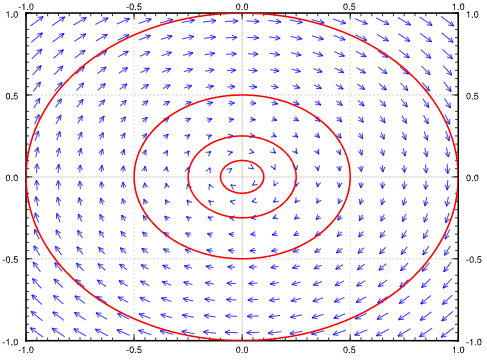
\includegraphics[scale=0.8]{Images/ODEPictures/phasePortrait6.png}
\begin{align*}
    &J(1,0)=\matrixx{0&1\\1&0}\Ra \lambda=\pm 1
\end{align*}
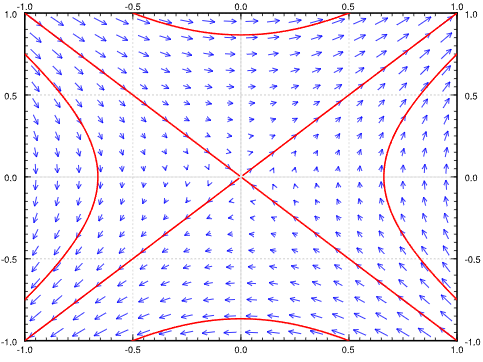
\includegraphics[scale=0.8]{Images/ODEPictures/phasePortrait7.png}\\
Combining the phase portraits gives a total system that looks something like\\
\centerline{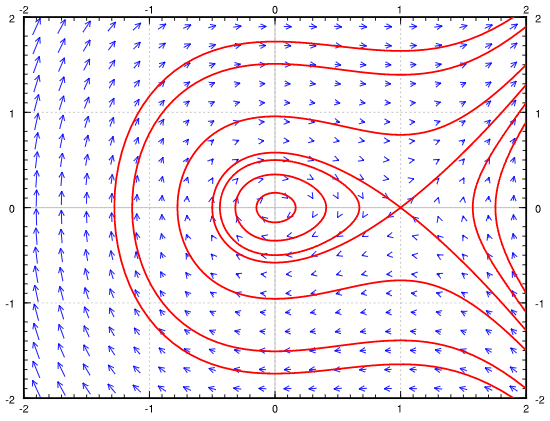
\includegraphics[scale=0.9]{Images/ODEPictures/phasePortrait8.png}}
